To perform a measurement in STXS bins, the first step is to construct a variable that can serve as a proxy for the transverse momentum (\ptw{}) of the associated vector boson. A straightforward approach is to use the \pt{} of the sub-sub-leading lepton (\ltwo{}), defined as the lepton with the largest angular separation from the opposite-sign lepton. However, this method has significant drawbacks. Notably, the second lepton is correctly identified in only about 85\% of events, resulting in a 15\% contamination from leptons not originating from the associated boson. Furthermore, due to the presence of an undetected neutrino, the full reconstruction of the $W$ boson's \pt{} is not possible.

An alternative, and ultimately preferred, approach is to train a regression neural network with a single output node to predict \ptw{}. The network is optimized to minimize the difference between its output (\ptr{}) and the true \ptw{}. The input features used for training the network are listed in Table~\ref{tab:regression_network_inputs} and can be seen in Appendix~\ref{app:stxs_input_plots}, and the network architecture is detailed in Table~\ref{tab:regression_network_architecture}.

\begin{table}
\centering
  \begin{tabular}{c||c}
  \hline
  \multicolumn{2}{c}{\textbf{Variable: Description}} \\
  \hline
  \multicolumn{2}{c}{
    \begin{tabular}{l@{: }l}
      $\Delta{\eta}_{\ell_{i}\ell_{j}}(i \neq j)$ & Pseduorapidity separation between lepton pairs \\
      $\Delta{\varphi_{\ell_{i}\ell_{j}}(i \neq j)}$ & Azimuthal separation between lepton pairs \\
      $\Delta{R_{\ell_{i}\ell_{j}}(i \neq j)}$ & Angular distance between lepton pairs \\
      $\Delta{m_{\ell_{i}\ell_{j}}(i \neq j)}$ & invariant masses of the lepton pairs \\
      $\pt^{\ell_{i}} (i = 0,1,2)$ & Lepton transverse momentum \\ 
      $\Delta{\varphi_{\ell_{i}\met}}$ & Azimuthal separation between each lepton and \met{} \\
      $\pt^{\ell\ell\ell}$ & Magnitude of the vectorial sum of lepton $\pt$ \\
      $\met$ & Missing transverse energy \\
      $\metsig$ & Significance of the missing transverse energy \\
    \end{tabular}
  } \\
  \hline
  \end{tabular}
  \caption{Input variables used for training regression ANN used to predict \ptv{}.}\label{tab:regression_network_inputs}
\end{table}

\begin{table}[htp]
\centering
  \begin{tabular}{c|c}
    \hline
    \textbf{Hyperparameter} & \zdom{} \\
    \hline
    \hline
    Batch Size & 4096 \\
    Epochs & 10000 \\
    k-Folds & 5 \\
    Training Size & 0.8 \\
    Validation Size & 0.1 \\
    Test Size & 0.1 \\
    Optimizer & Nadam \\
    Learning Rate & $1 \times 10^{-5}$ \\
    Loss Function & Huber \\
    Number of Layers & 4 \\
    Neurons per Layer & 93, 92, 75, 37 \\
    Dropout After Layer & 0.1, 0.1, 0.1, 0.1 \\
    Activation Functions & Swish \\
    Kernel Initializer & Glorot Normal \\
  \end{tabular}
  \caption{Summary of the optimal hyperparameters for the regression ANN.}\label{tab:regression_network_architecture}
\end{table}

Correlations between the \pt{} of the \ltwo{} lepton and the true \ptw{}, as well as between the regression output \ptr{} and the true \ptw{}, are shown in Figure~\ref{fig:regression_ptw_correlation}. These plots demonstrate that the regression output exhibits a stronger correlation with the true \ptw{} than the \pt{} of the \ltwo{} lepton, indicating that the regression network provides a more accurate proxy for the associated boson's transverse momentum.

\begin{figure}[htbp]
    \centering
    \subfloat[$\pt^{\ltwo{}}$ vs \ptw{}]{
      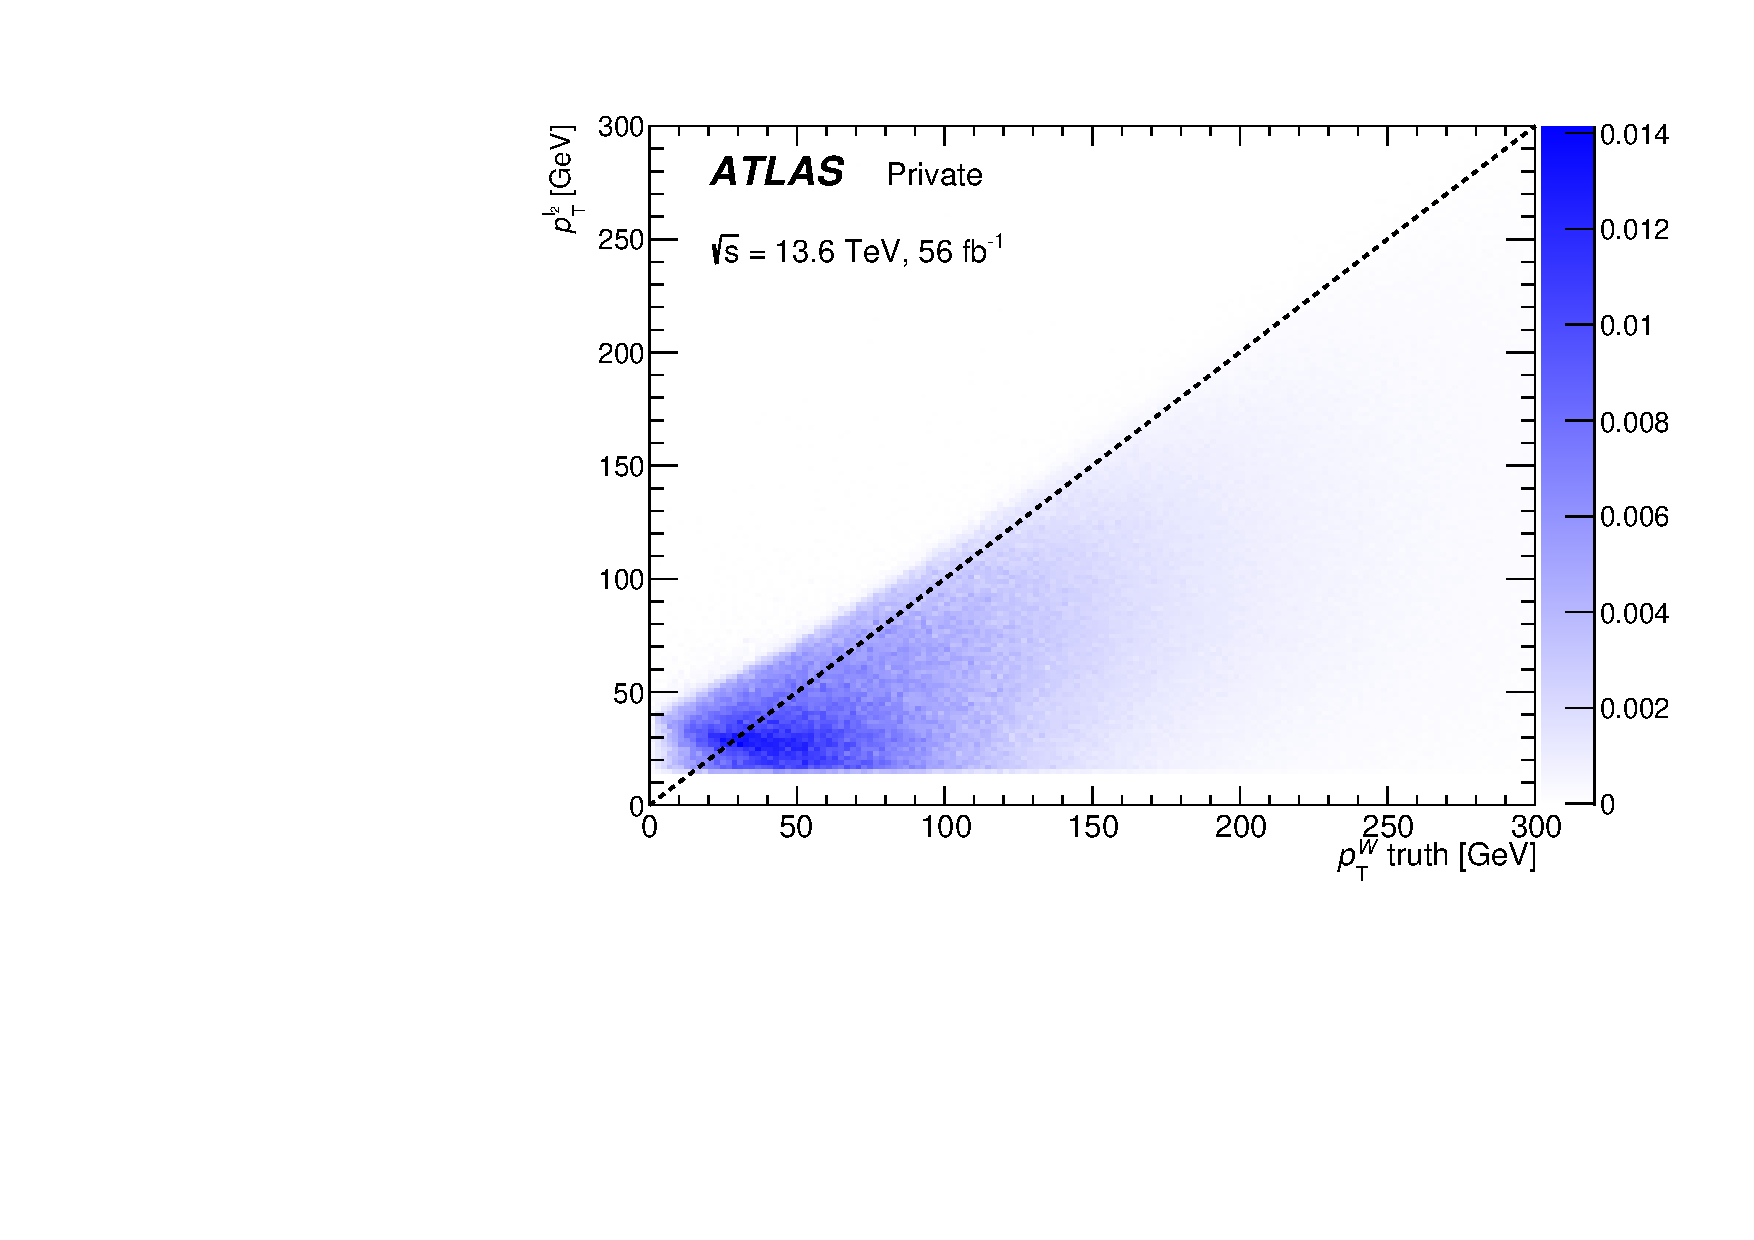
\includegraphics[width=0.48\linewidth]{figures/stxs/truth_vs_ptl2.pdf}
    }
    \subfloat[$\pt^{R}$ vs \ptw{}]{
      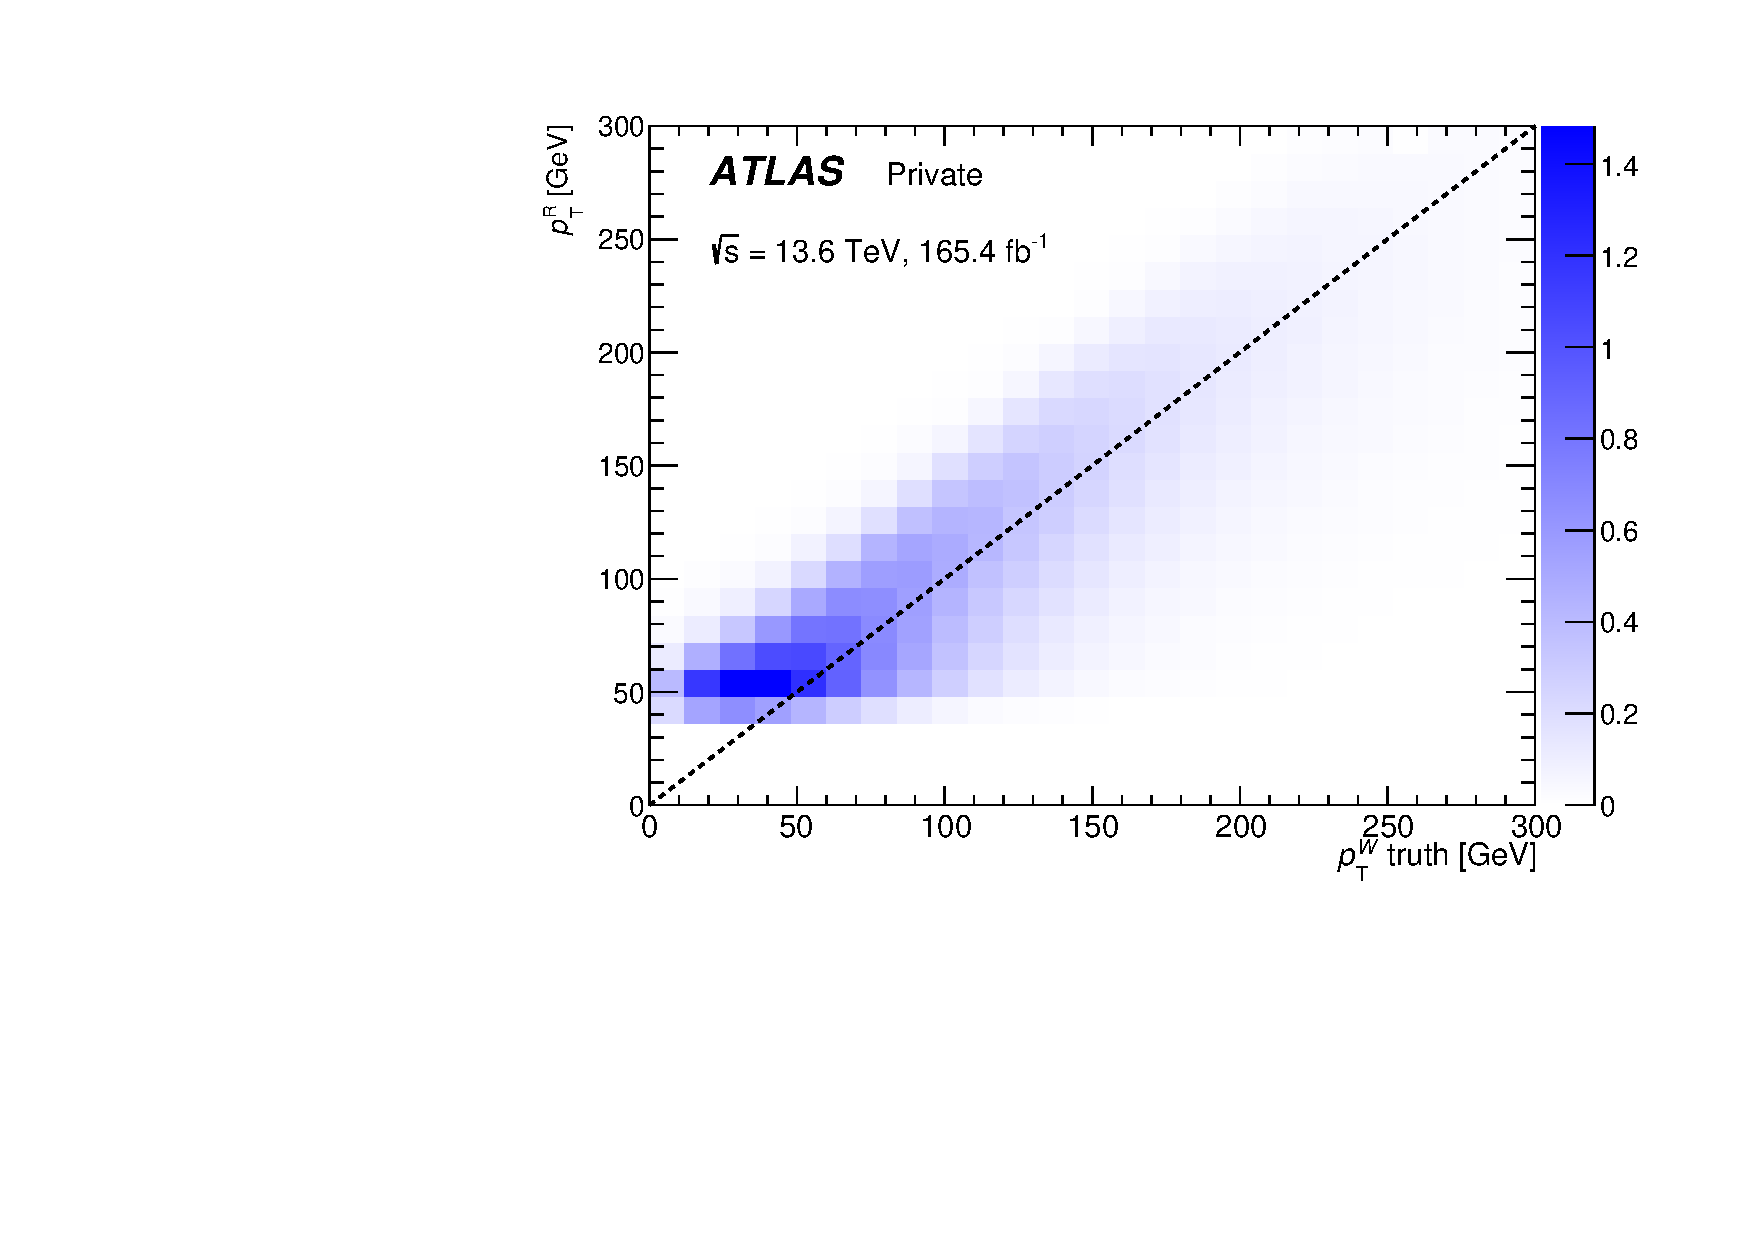
\includegraphics[width=0.48\linewidth]{figures/stxs/truth_vs_regressor.pdf}
    }
    \caption{Correlations between the \pt{} of the \ltwo{} lepton and truth \ptw{} (left) and regression output and true \ptw{} (right). Perfect agreement is represented by the black dashed line on the plot. The regressed \pt{} exhibits a stronger correlation with the true \ptv{} indicating it is a more accurate proxy than the other.}\label{fig:regression_ptw_correlation}
\end{figure}

Figure~\ref{fig:nndiscriminant_vs_ptr} shows the distributions of the three STXS categories plotted against the neural network discriminant and the regression output \ptr{}. The classification and regression neural networks are uncorrelated, allowing us to divide the inclusive signal region into subregions enriched in each STXS category for use in the statistical analysis. From these distributions, it is clear that the STXS regions are not perfectly pure within their respective \ptv{} bins, as the regression output is not exact. To better isolate the different STXS bins and their characteristic peaks, we define cut values at 80~GeV and 160~GeV, resulting in three distinct regions optimized to maximize the signal purity in each.

\begin{figure}[htbp]
    \centering
    \subfloat[$\ptw{} < 75$~GeV]{
      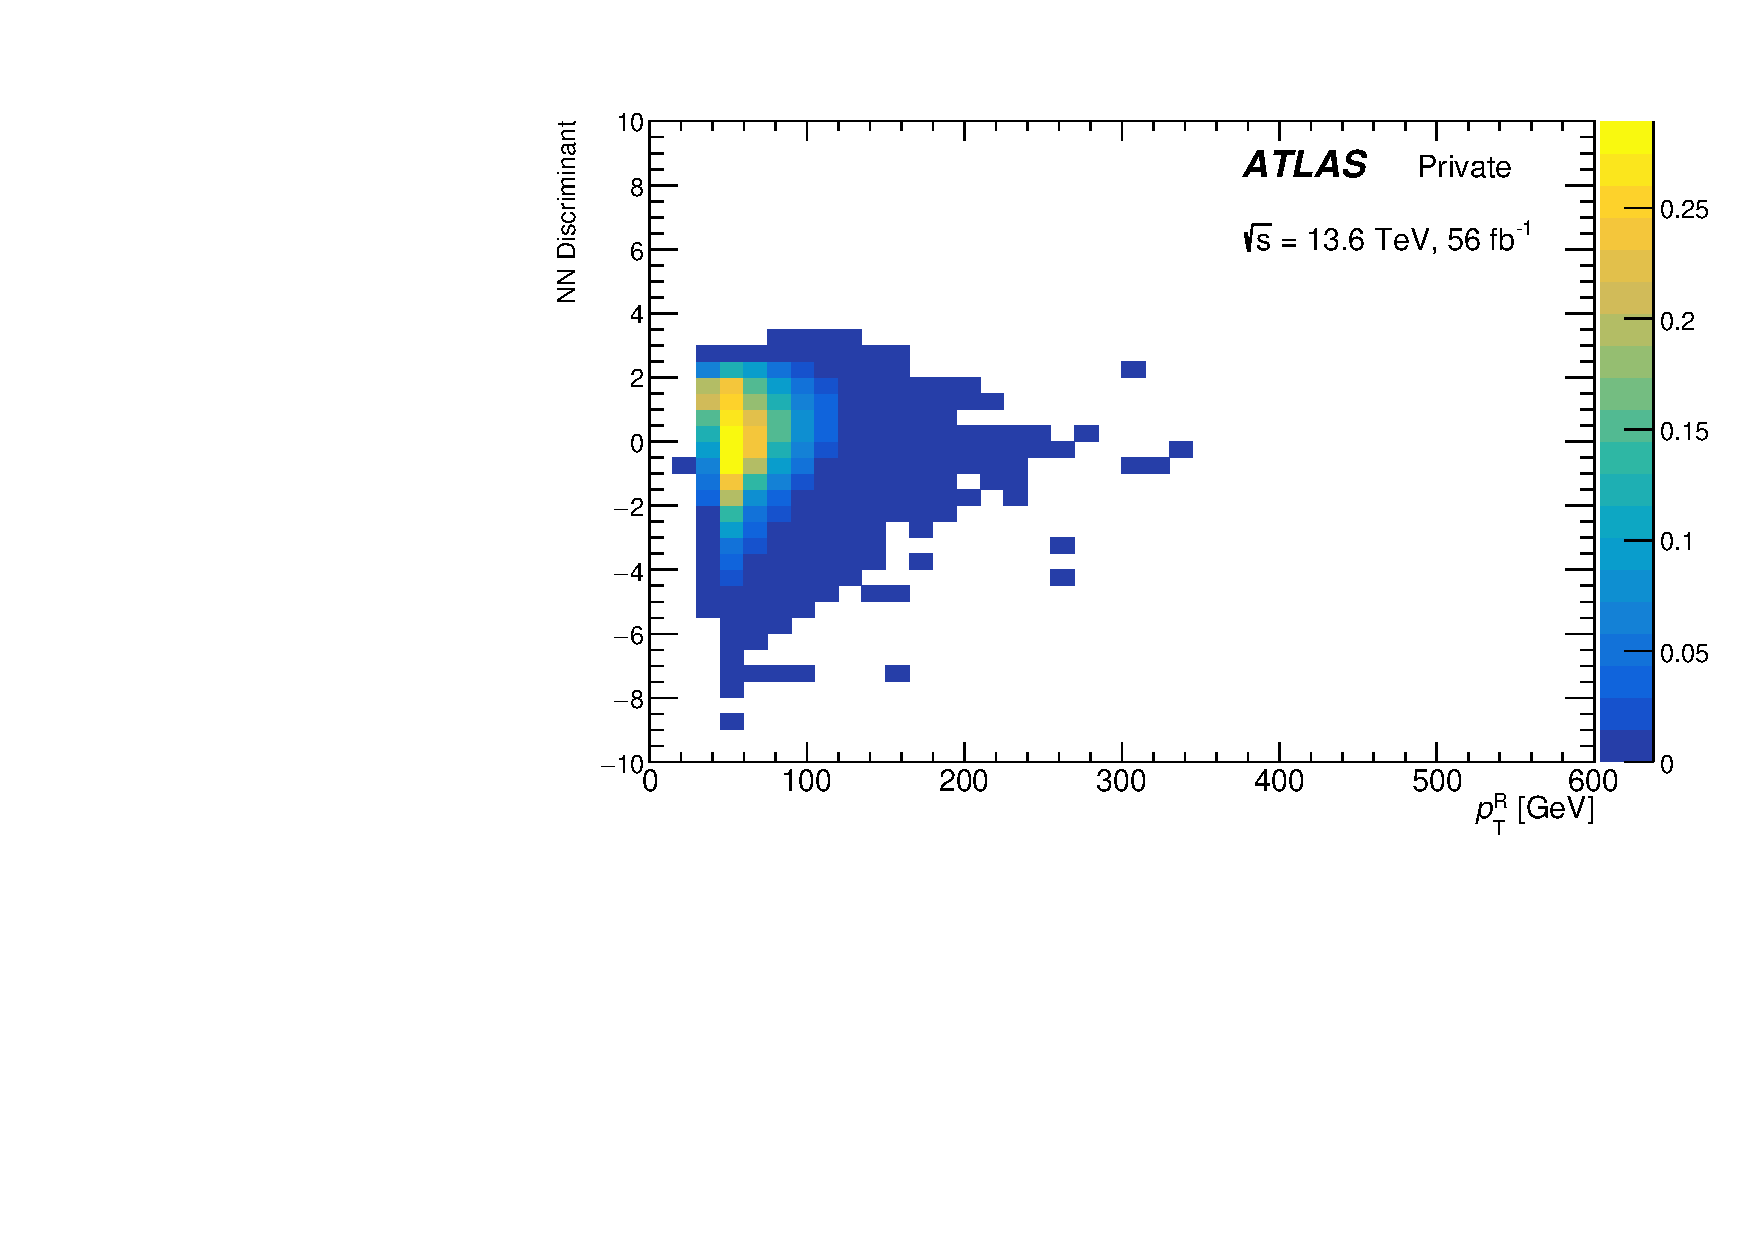
\includegraphics[width=0.48\linewidth]{figures/stxs/plot_75.pdf}
    }
    \subfloat[$75~\mathrm{GeV} <\ptw{} < 150$~GeV]{
      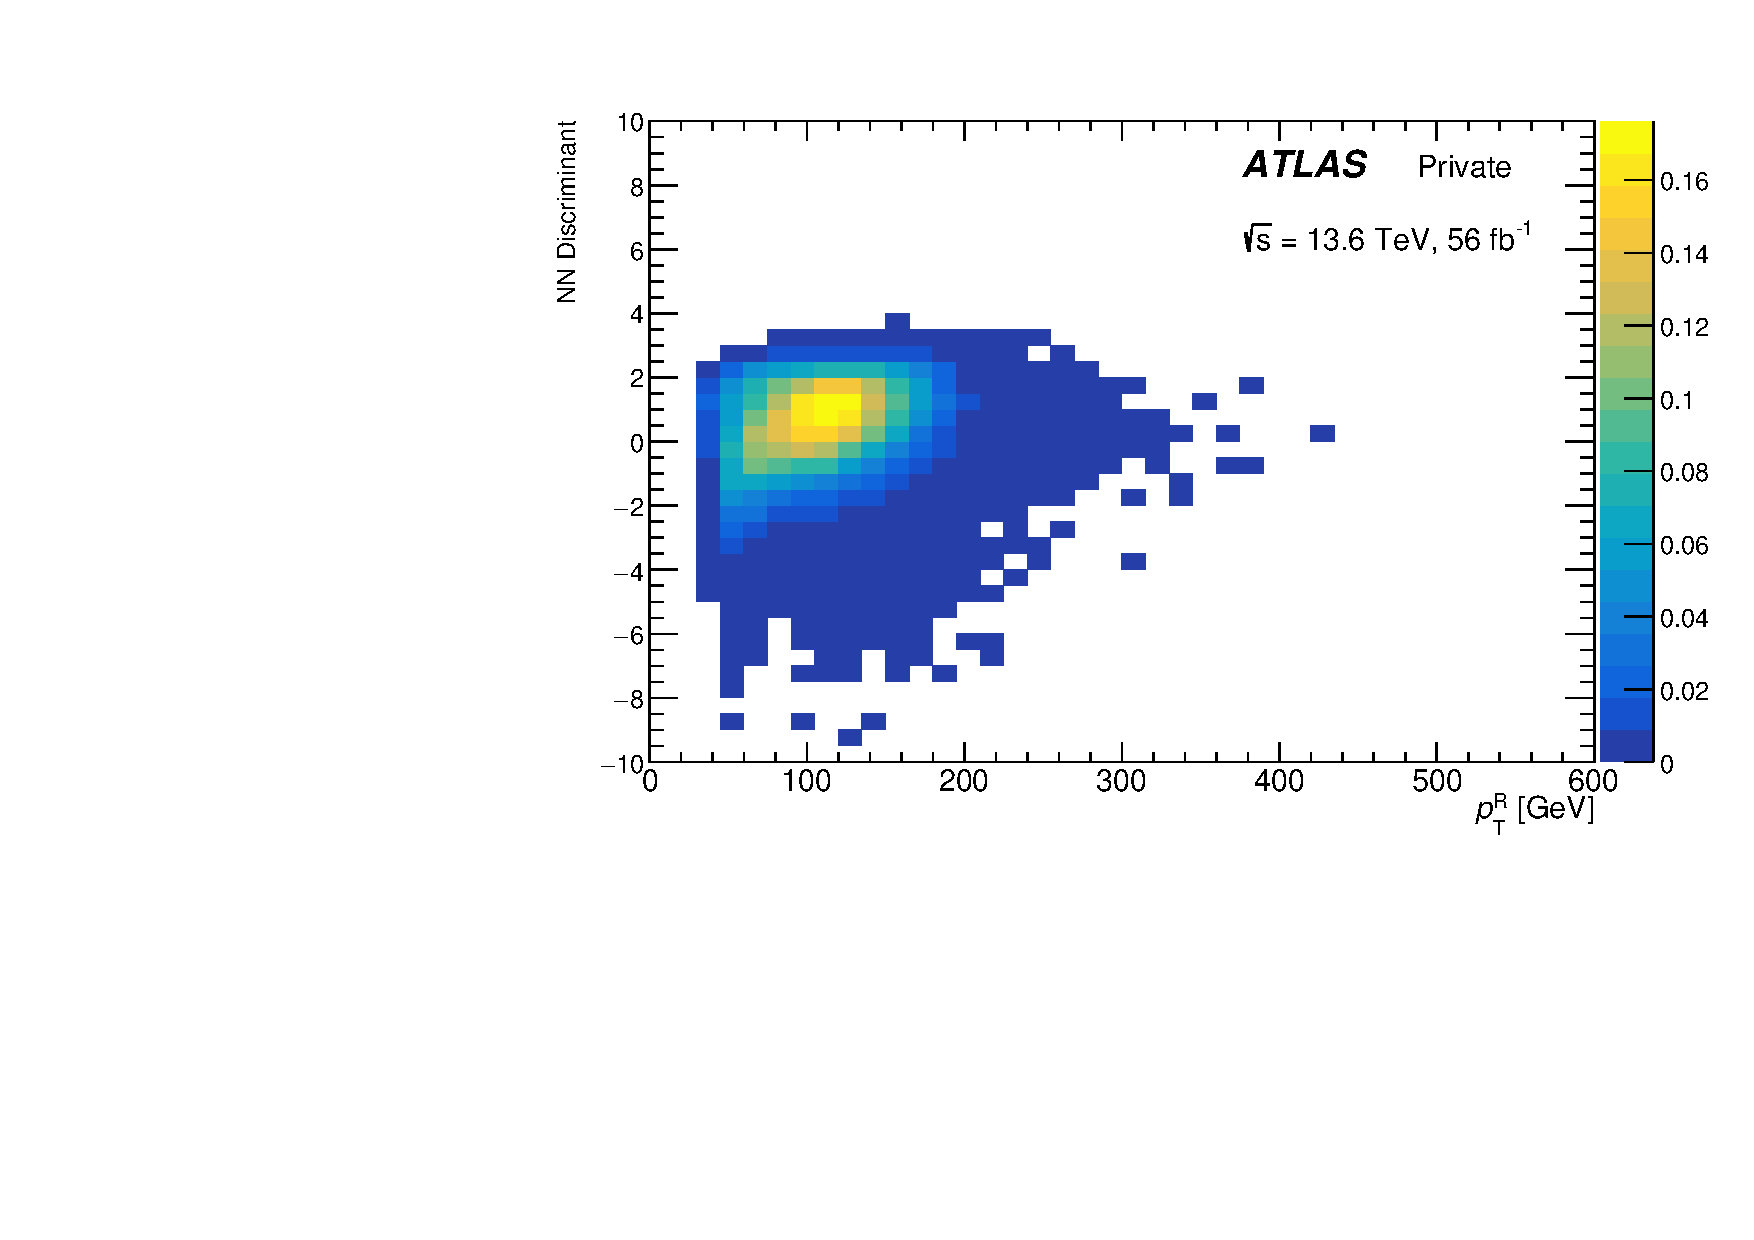
\includegraphics[width=0.48\linewidth]{figures/stxs/plot_75_150.pdf}
    }
    \hfill
    \subfloat[$\ptw{} > 150$~GeV]{
      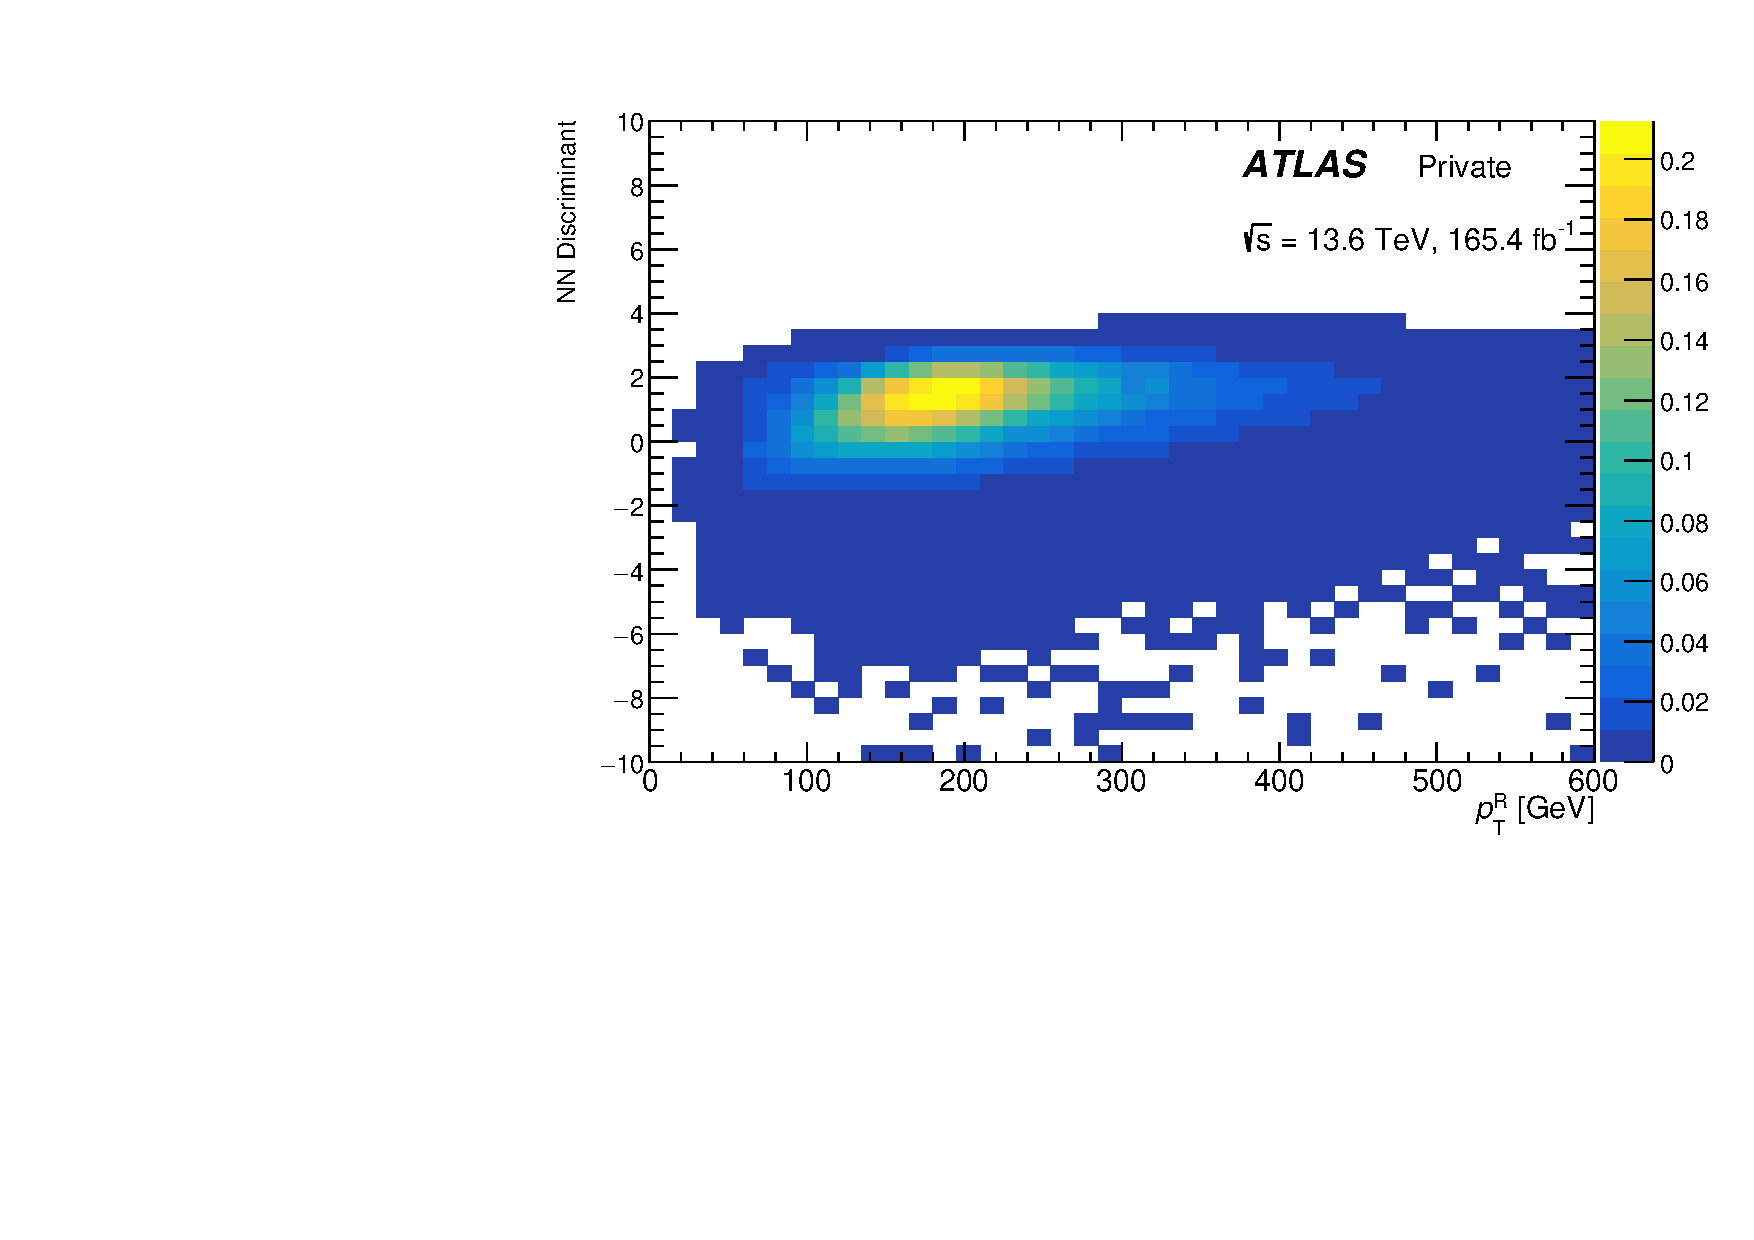
\includegraphics[width=0.48\linewidth]{figures/stxs/plot_150.pdf}
    }
    \caption{Plots of the neural network discriminant versus \ptr{}. Panel (a) shows the distribution for the 0--75~GeV bin, (b) for the 75--150~GeV bin, and (c) for the 150+~GeV bin. Leakage between bins is observed in all plots, motivating the implementation of \ptr{} cuts to better separate the peaks of these three distributions.}\label{fig:nndiscriminant_vs_ptr}
\end{figure}

This \ptr{} variable has been validated in our $WZ$ CR's (Figure~\ref{fig:WZ_regressor_val}) and VR's (Figure~\ref{fig:VR_regressor_val}), where good data-MC agreement is observed.

\begin{figure}[htbp]
    \centering
    \subfloat[$\pt^{R}$ in $WZ 0$ jets CR]{
      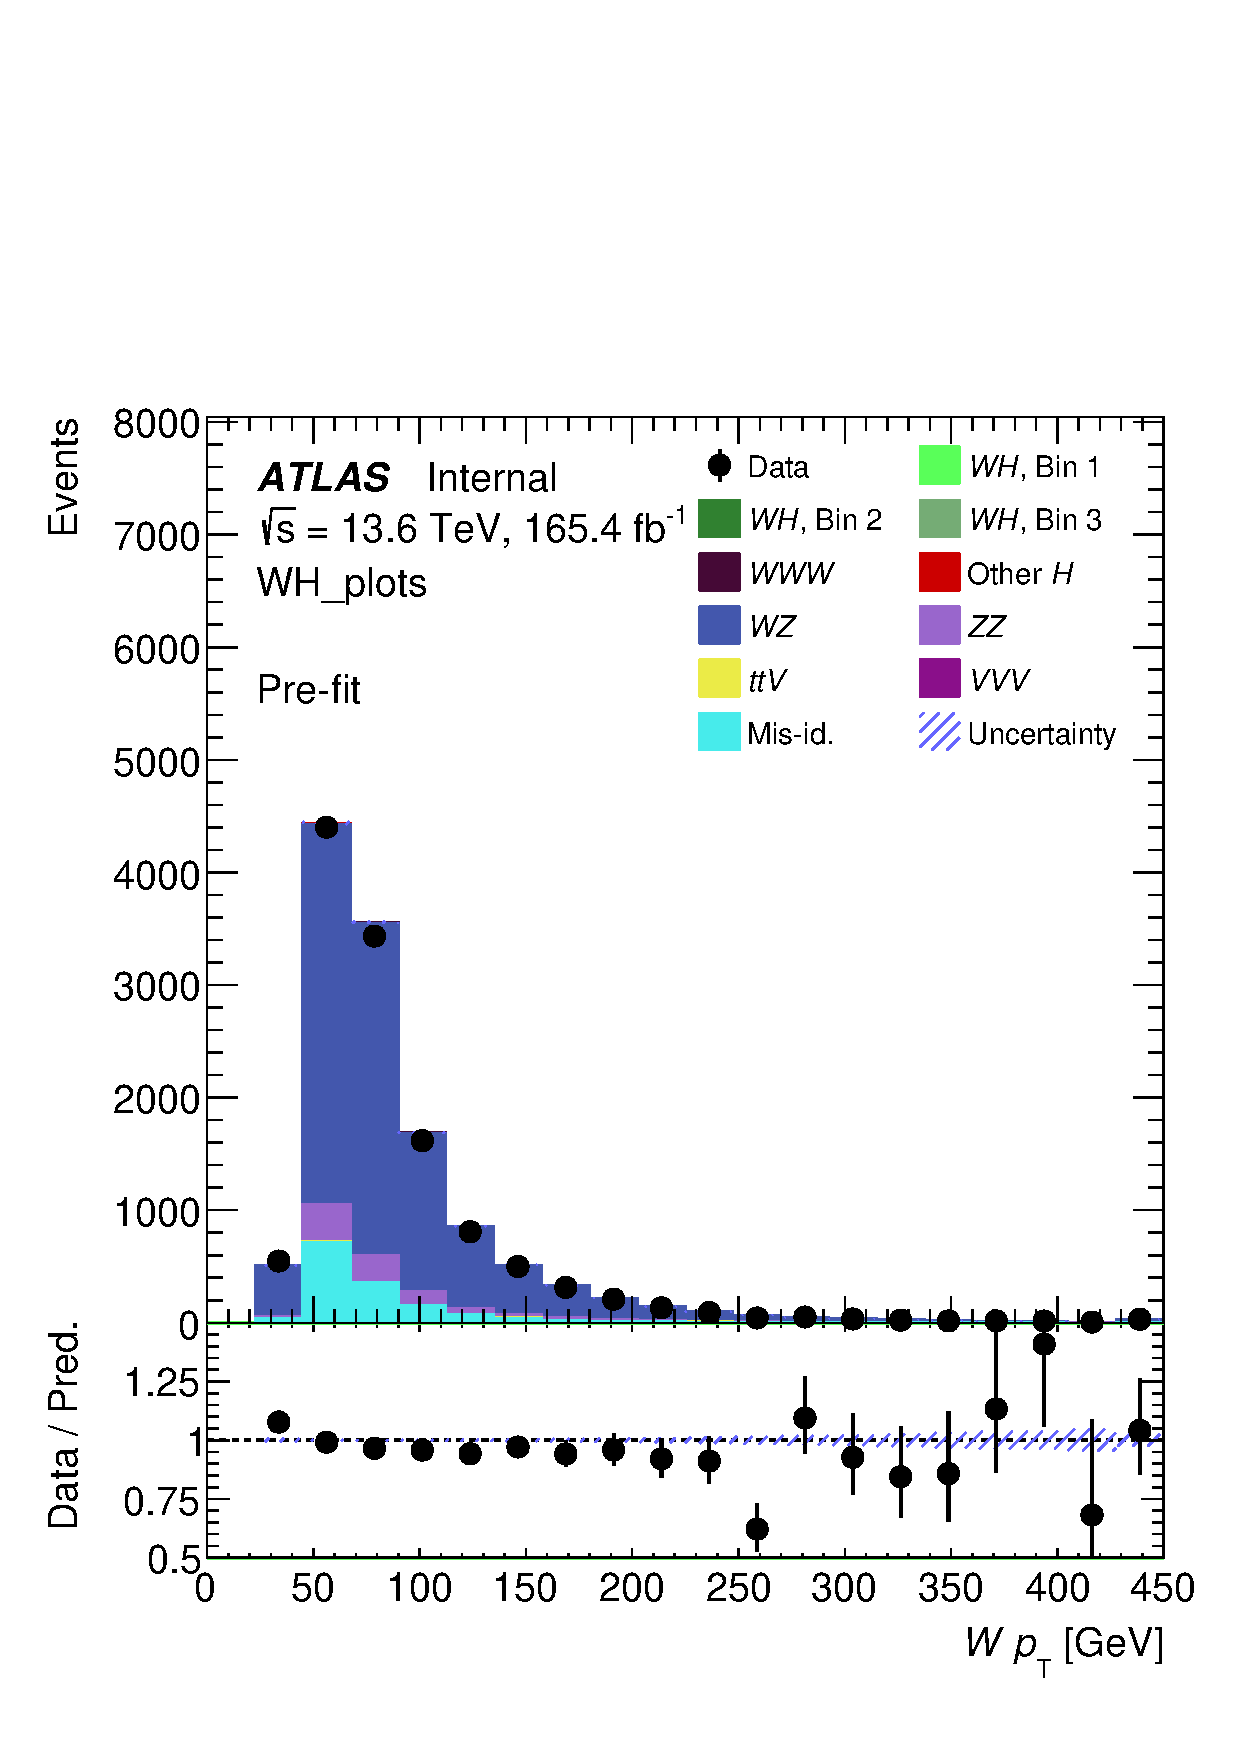
\includegraphics[width=0.48\linewidth]{figures/stxs/WZCR_0jet_regressed_WPt.pdf}
    }
    \subfloat[$\pt^{R}$ in $WZ 1$ jet CR]{
      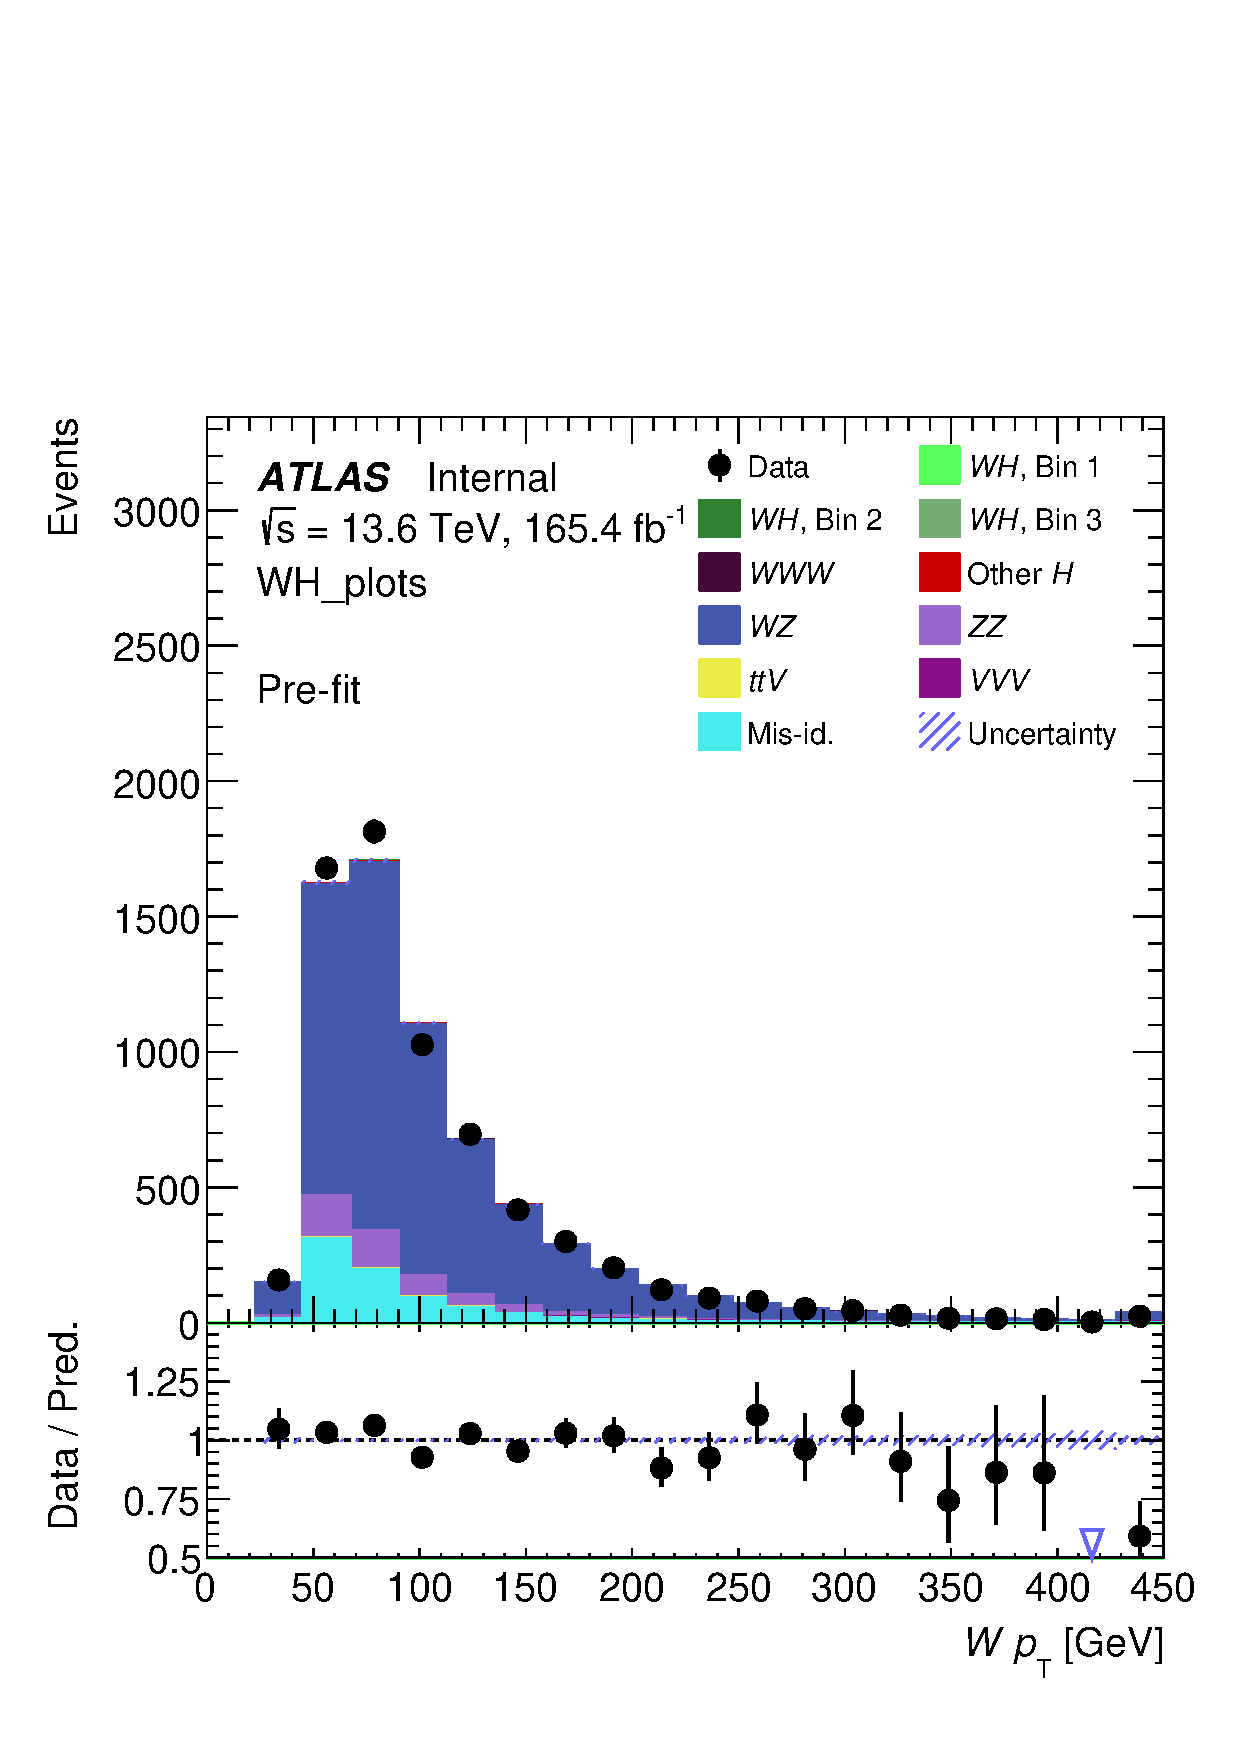
\includegraphics[width=0.48\linewidth]{figures/stxs/WZCR_1jet_regressed_WPt.pdf}
    }
    \hfill
    \subfloat[$\pt^{R}$ in $WZ 2+$ jets CR]{
      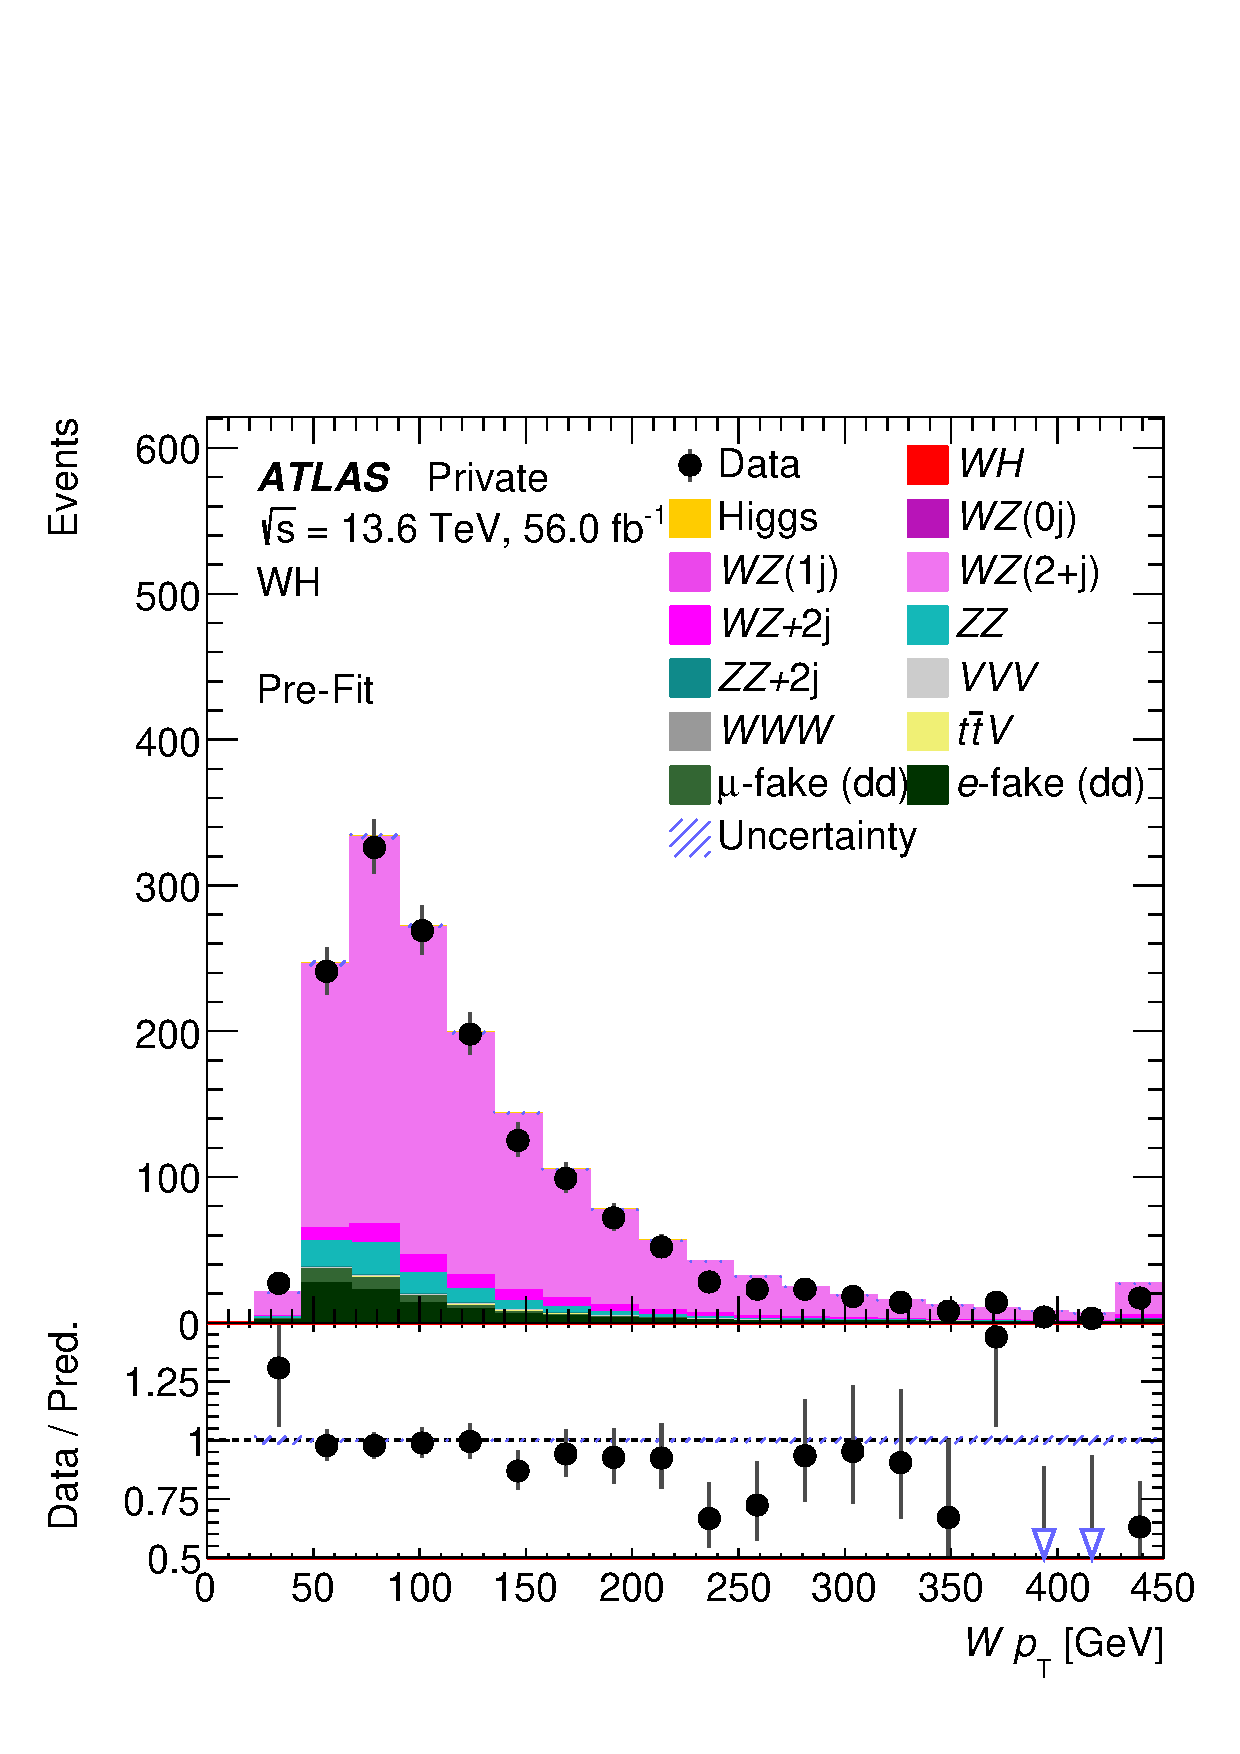
\includegraphics[width=0.48\linewidth]{figures/stxs/WZCR_2jet_regressed_WPt.pdf}
    }    
    \caption{Validation plots of the regression NN in the WZ CR's. Good data-MC simulation agreement is seen. WZ NF's are not applied.}\label{fig:WZ_regressor_val}
\end{figure}

\begin{figure}[htbp]
    \centering
    \subfloat[$\pt^{R}$ in \zdom{} VR]{
      
\includegraphics[width=0.48\linewidth]{figures/stxs/Zdominated_VR_regressed_WPt.pdf}
    }
    \subfloat[$\pt^{R}$ in \zdom{} Top VR]{
      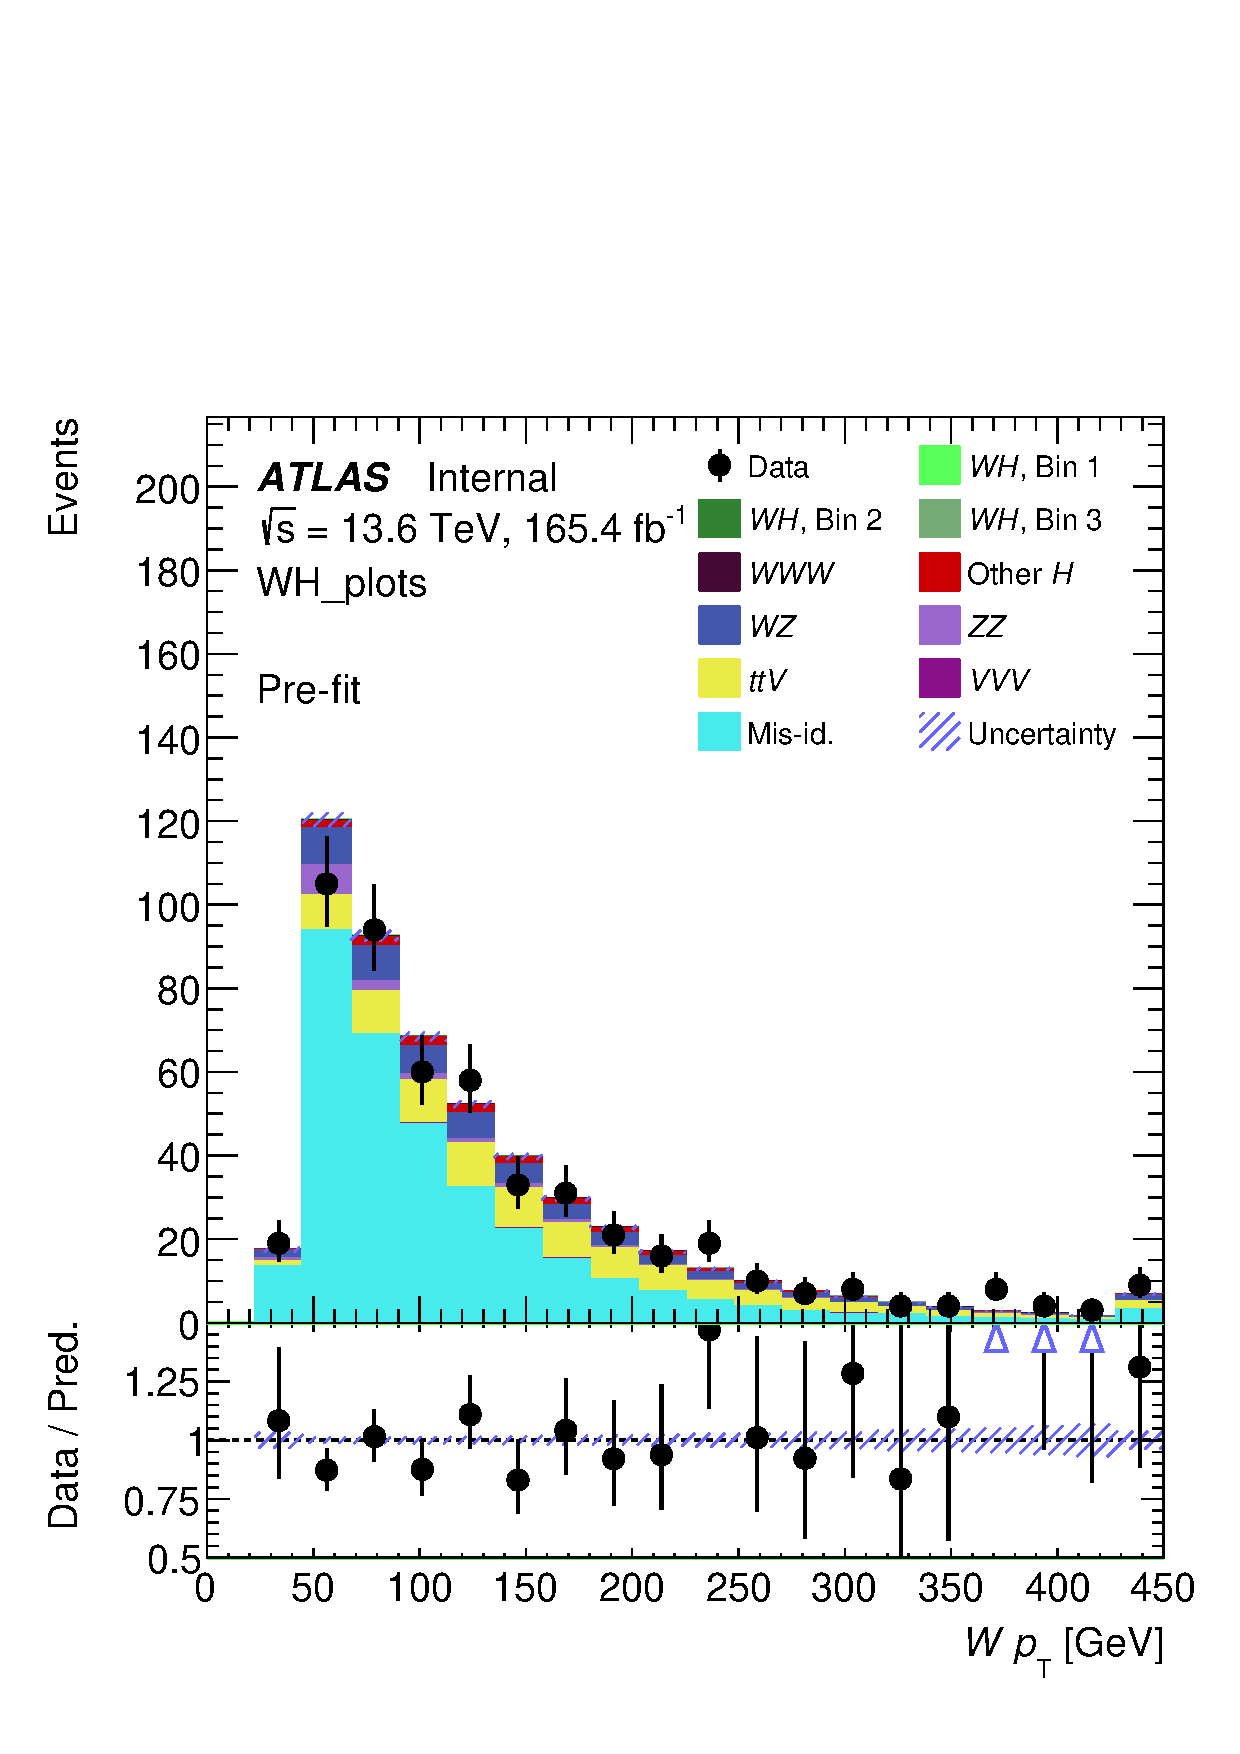
\includegraphics[width=0.48\linewidth]{figures/stxs/Zdominated_top_VR_regressed_WPt.pdf}
    }
    \hfill
    \subfloat[$\pt^{R}$ in \zdep{} Top VR]{
      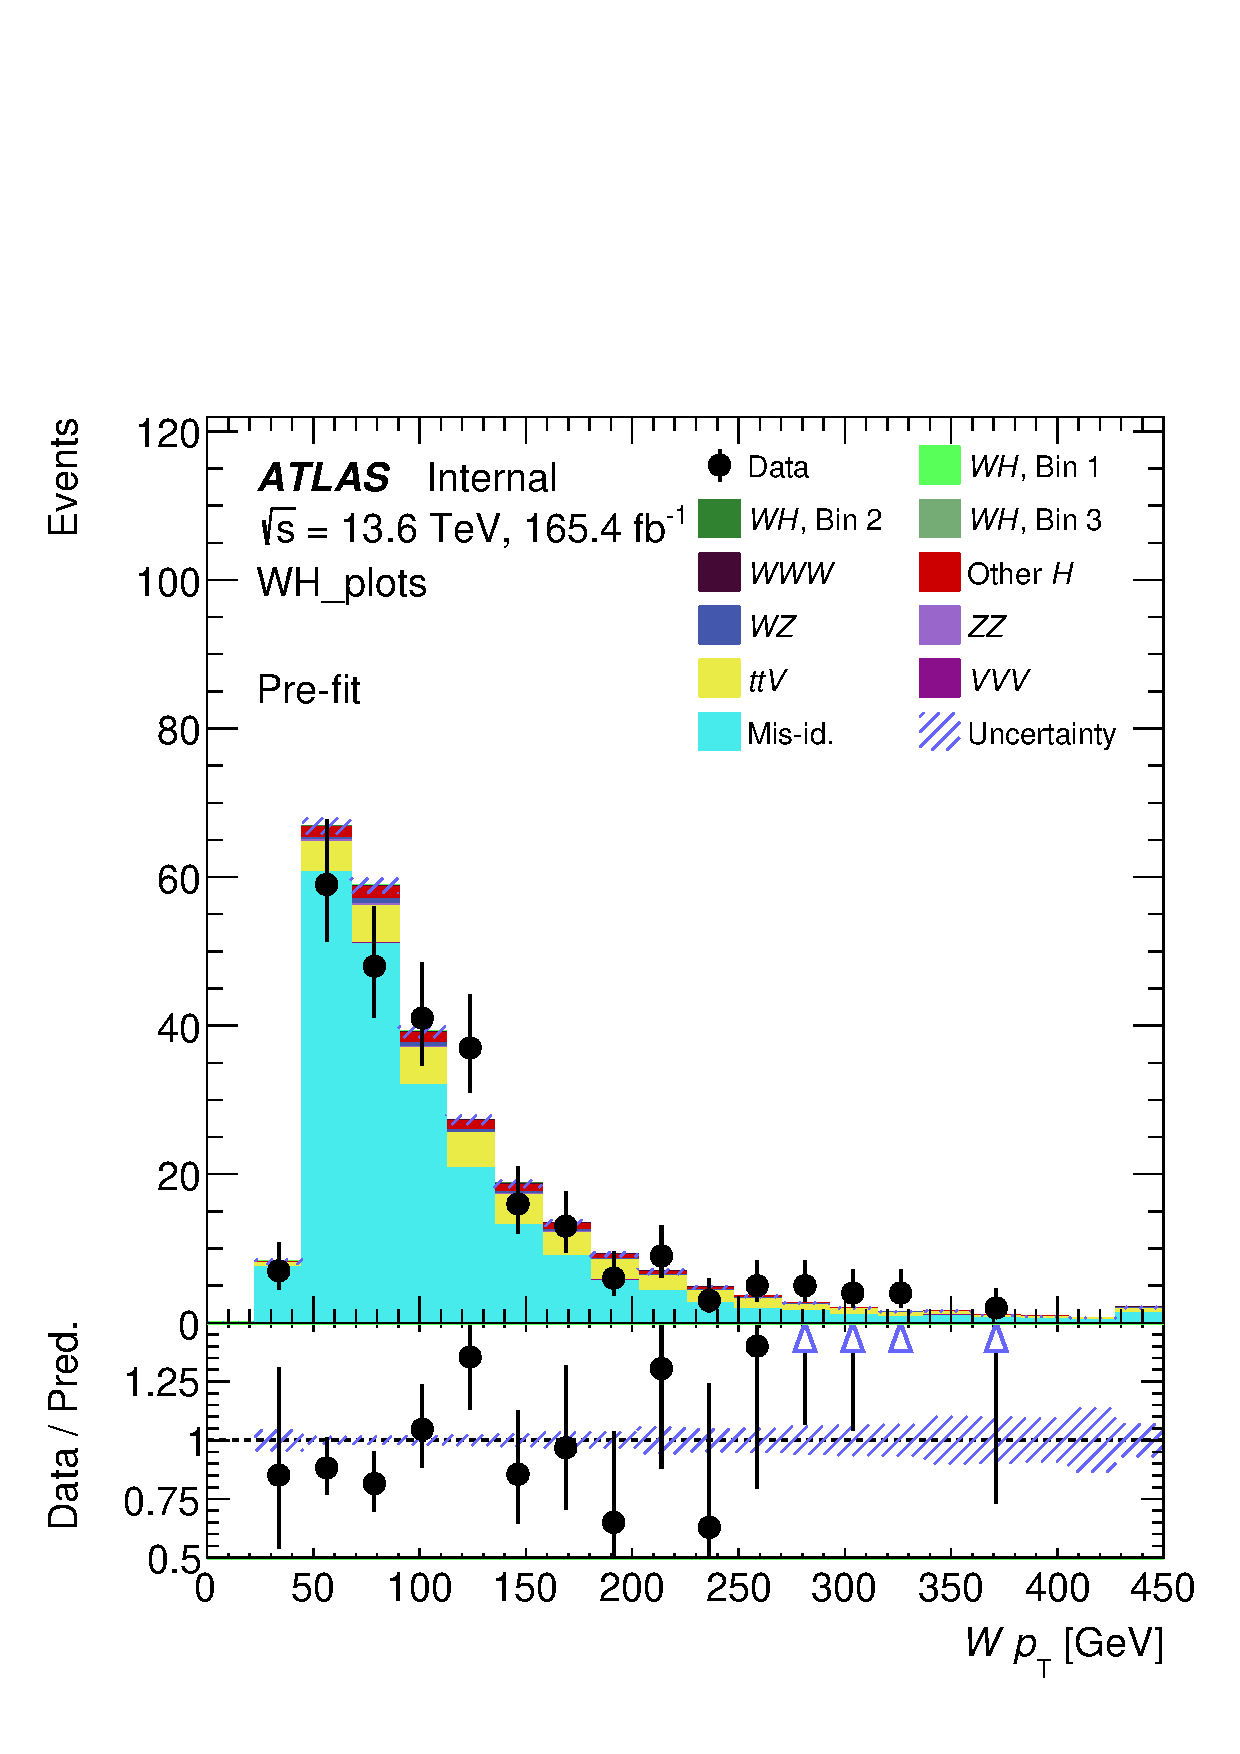
\includegraphics[width=0.48\linewidth]{figures/stxs/Zdepleted_top_VR_regressed_WPt.pdf}
    }    
    \caption{Validation plots of the regression NN in the WZ CR's. Good data-MC simulation agreement is seen.}\label{fig:VR_regressor_val}
\end{figure}